\documentclass[11pt,a4paper]{article}
\usepackage{fontspec}
\setmainfont{TeX Gyre Pagella}
\newfontfamily\headfont{Inter}[UprightFont=*-ExtraBold,BoldFont=*-ExtraBold,Extension=.otf,Path=/usr/share/fonts/opentype/inter/]
\usepackage[a4paper,margin=2.3cm]{geometry}
\usepackage{graphicx}
\graphicspath{ {../blog/} }
\usepackage{booktabs,float,caption,array,xcolor}
\usepackage[hidelinks]{hyperref}
\usepackage{titlesec}
\usepackage{setspace}
\usepackage[round]{natbib}
\setstretch{1.05}
\renewcommand{\topfraction}{0.9}
\renewcommand{\bottomfraction}{0.8}
\renewcommand{\textfraction}{0.1}
\renewcommand{\floatpagefraction}{0.75}
\setlength{\parindent}{0pt}
\setlength{\parskip}{0.55em}
\titleformat{\section}{\headfont\Large}{\thesection}{0.8em}{}
\titleformat{\subsection}{\headfont\large}{\thesubsection}{0.8em}{}
\captionsetup{font=small,labelfont=bf}
\urlstyle{same}
\hypersetup{pdftitle={How Deep Is the Sea?},pdfauthor={Tristan Hotham}}

\begin{document}
\begin{center}
{\Large\bfseries How Deep Is the Sea?\\[2pt] Ocean Depth, Trenches and the Unmapped Sea Floor, from Open Data\par}
\vspace{1.2em}
{\large Tristan Hotham\par}
\vspace{0.3em}
{\small Independent researcher\\
ORCID: 0000-0003-4931-9349\\
DOI: 10.5281/zenodo.23850291\par}
\vspace{0.8em}
2026
\end{center}

\begin{quote}
\small
\begin{center}\textbf{Abstract}\end{center}
I describe the depth of the world ocean from the open AWS Terrain Tiles, whose sea floor comes from ETOPO1, GEBCO and SRTM15+, using the zoom 4 level of the tiles as a 4,096 by 4,096 Web Mercator grid of about 9.8 km at the equator, with every cell weighted by its true area and by the share of it that is sea. The sea covers 362.9 million km², 71.2\% of the Earth, with a mean depth of 3,675 m, a median of 4,089 m and a volume of 1.33 billion km³, close to published estimates. Continental shelf shallower than 200 m covers 7.7\% of the sea floor, slopes, rises and ridges between 200 and 3,000 m 17.3\%, the abyssal depths between 3,000 and 6,000 m 74.1\% (more than half of the planet's surface) and the hadal trenches below 6,000 m 1.0\%. The Pacific is the deepest ocean on average (3,943 m) and the Arctic the shallowest (1,205 m). Comparing the grid with published surveys of 14 of the deepest places shows how much a 10 km grid smooths the trenches: its deepest Mariana cell is 671 m shallower than the 10,935 m measured at the Challenger Deep, its deepest cell overall lies in the Tonga Trench, and in 4 trenches it is deeper than any measured depth, pointing to errors in the source grids. National waters cover 39\% of the sea but hold 37\% of the floor deeper than 6,000 m. Finally I set these numbers against the Seabed 2030 project's estimate that only 28.7\% of the floor is mapped to modern standards. An interactive map draws the same tiles at every zoom with a depth readout for any point.

\textbf{Keywords:} bathymetry; ocean depth; hypsometry; ocean trenches; hadal zone; seamounts; exclusive economic zones; GEBCO; ETOPO1; Seabed 2030; open data; mapping
\end{quote}

\section{Introduction}
Most of the Earth's surface is sea floor, and most of the sea floor is deep. Yet it is the least well known surface in the solar system that we can reach: far more of it has been estimated than measured. Global grids of ocean depth, such as ETOPO1 \citep{etopo1}, the GEBCO grid \citep{gebco} and SRTM15+ \citep{srtm15}, combine ship soundings with depths predicted from satellite measurements of the height of the sea surface, which bulges over seamounts and sags over trenches. The Seabed 2030 project, which compiles GEBCO, reported in 2026 that 28.7\% of the ocean floor is mapped to modern standards \citep{seabed2030}.

The same global grids are built into the open terrain tiles first made by Mapzen and now hosted by Amazon \citep{terraintiles, joerd}, the source a sibling study used for the land \citep{worldterrain}. This study turns them to the sea. It measures the depth of the world ocean, by ocean, by sea and by national waters, from the coarsest level of the tiles, weighting every cell by its true area and stating what a 10 km grid can and cannot see. It compares the grid with published surveys of the deepest places \citep{greenaway, bongiovanni, stewart}. And it builds an interactive map (\url{https://maps.tristanhotham.com/ocean-depth/}) that decodes the tiles in the browser at every zoom, with depth tints, shaded relief, depth bands, the trenches, named seamounts and a readout of the depth of any point.

\section{Data}
Table~\ref{tab:sources} lists the sources. The AWS Terrain Tiles store a height in metres in the colour of each pixel of a web map tile, in the Terrarium encoding: height $= R \times 256 + G + B/256 - 32{,}768$. Under the sea their sources are ETOPO1, GEBCO and SRTM15+ \citep{joerd}; all three blend sparse ship soundings with depths predicted from satellite altimetry, so away from survey tracks their detail is limited to roughly 10 to 20 km. The polar cap north of 85.05° N, outside Web Mercator, comes from ETOPO10, a 10 arc minute grid derived from ETOPO1.

Natural Earth supplies land, lakes, countries, place and marine names, and a set of bathymetric polygons (areas deeper than 0, 200, 1,000 m and so on) used here as a cross-check \citep{naturalearth}. Marine Regions supplies the IHO sea areas \citep{iho, marineregions}, the Exclusive Economic Zones, joint regimes and overlapping claims, and the gazetteer of undersea feature names, from which I take 2,000 named seamounts, 219 guyots, 330 knolls, 51 trenches, 36 deeps and other features, 5,638 in all. The global seamount census of \citet{kw2011}, which lists 24,646 likely seamounts, could not be downloaded from its host and is cited only. Measured depths of the deepest places come from the papers in Table~\ref{tab:trenches}.

\begin{table}[tbp]\centering\small\caption{Sources, what was used and licences.}\label{tab:sources}\begin{tabular}{>{\raggedright\arraybackslash}p{3.8cm}>{\raggedright\arraybackslash}p{7.4cm}>{\raggedright\arraybackslash}p{3.2cm}}\toprule Source & Used & Licence\\\midrule
AWS Terrain Tiles (Terrarium; sea floor from ETOPO1, GEBCO, SRTM15+) & Zoom 4 grid for statistics; all zooms on the map & Per source; mostly public domain\\
ETOPO10 (from ETOPO1) & Arctic north of 85.05 N; Antarctic interior for the Earth histogram & Public domain\\
Natural Earth & Land, lakes, countries, places, marine names; bathymetry polygons as a check & Public domain\\
Marine Regions (VLIZ) & IHO sea areas; 267 EEZs, joint regimes and claims; 5,638 undersea feature names & CC BY 4.0\\
Published surveys and Wikipedia & Depths of the deepest places (Table~\ref{tab:trenches}) & Cited; Wikipedia CC BY-SA 4.0\\
Seabed 2030 / GEBCO & Share of the floor mapped to modern standards & Cited\\
\bottomrule\end{tabular}\end{table}

\section{Methods}
\subsection{The depth grid}
The 256 zoom 4 tiles were mosaicked into one Web Mercator grid of 4,096 by 4,096 cells, 9.8 km across at the equator and 4.9 km at 60°. 13 cells that differed from the median of their neighbours by more than 2,500 m in shallow ground were replaced by that median; trenches, which are tens of kilometres wide, always have deep neighbours and are untouched. Each cell's area was computed exactly for its band of latitude on a sphere of radius 6,371 km.

\subsection{What counts as sea}
Natural Earth's 1:10m countries and lakes were rasterised at twice the grid's resolution, giving each cell the share of it that is sea. Only water joined to the world ocean counts: the Caspian, which Natural Earth does not list as a lake, was removed by hand, and the Black Sea, joined to the Mediterranean only by the narrow Bosporus, was kept. A sea cell's depth is minus its height, and sea cells whose 10 km average is above sea level count as 0 m deep. Antarctica's floating ice shelves are land in Natural Earth, so the sea beneath them, roughly 1.5 million km², is missing. The Arctic north of 85.05° N adds 0.9 million km² from ETOPO10.

\subsection{Oceans, seas and national waters}
The 101 IHO sea areas that hold sea cells were rasterised in the same way, sub-areas over their parents, and cells outside every polygon given the nearest area. They are grouped into five oceans: the Southern Ocean is the IHO's sea south of 60° S; the Arctic includes the Greenland, Norwegian, Barents, Kara, Laptev, East Siberian, Chukchi and Beaufort Seas and Baffin and Hudson Bays; the Indian Ocean includes the Red Sea, the Persian Gulf, the Great Australian Bight and the Malacca Strait; and the Pacific includes the seas of the East Indian Archipelago. National waters are the Marine Regions Exclusive Economic Zones, joint regimes and whole overlapping claims (267 zones that hold sea cells), grouped where useful by the adjective in their name (so that, for example, all French zones form one group).

\subsection{Statistics and checks}
Shares are of area. Means and volumes weight each cell by its sea area; medians come from 1 m bins. For each trench I took the deepest sea cell inside a box drawn round it, and compared it with the published depth of its deepest point. The profile through the Mariana Trench samples the grid bilinearly every kilometre along 142.6° E. As a check, I measured on the ellipsoid the area of each of Natural Earth's bathymetric polygons and compared it with the grid (Table~\ref{tab:ne}).

\section{Results}
\subsection{The shape of the sea floor}
The sea covers 362.9 million km² of the grid, 71.2\% of the Earth's surface. Its mean depth is 3,675 m and its median 4,089 m; the volume of water above the floor is 1.33 billion km³. \citet{charette} found 3682.2 m and 1.332 billion km³ from a finer grid; the small difference is about what the coarse grid, the missing sea under the ice shelves and the choice of coastline would lead one to expect.

The floor is overwhelmingly deep (Figure~\ref{fig:bands}). Only 7.7\% lies on the continental shelf above 200 m, 27.8 million km². The band from 200 to 3,000 m, the continental slopes and rises and the shallower parts of the mid-ocean ridges, takes 17.3\%. The abyssal depths between 3,000 and 6,000 m take 74.1\%, 268.8 million km², more than half of the whole planet's surface (52.7\%); the single most common band is 4,000 to 5,000 m, with 31.7\% of the floor. The hadal zone below 6,000 m, almost all of it in trenches, is 1.00\% of the sea floor, about 3,632,872 km² on this grid, and 0.12\% lies deeper than 7,000 m.

\begin{figure}[tbp]\centering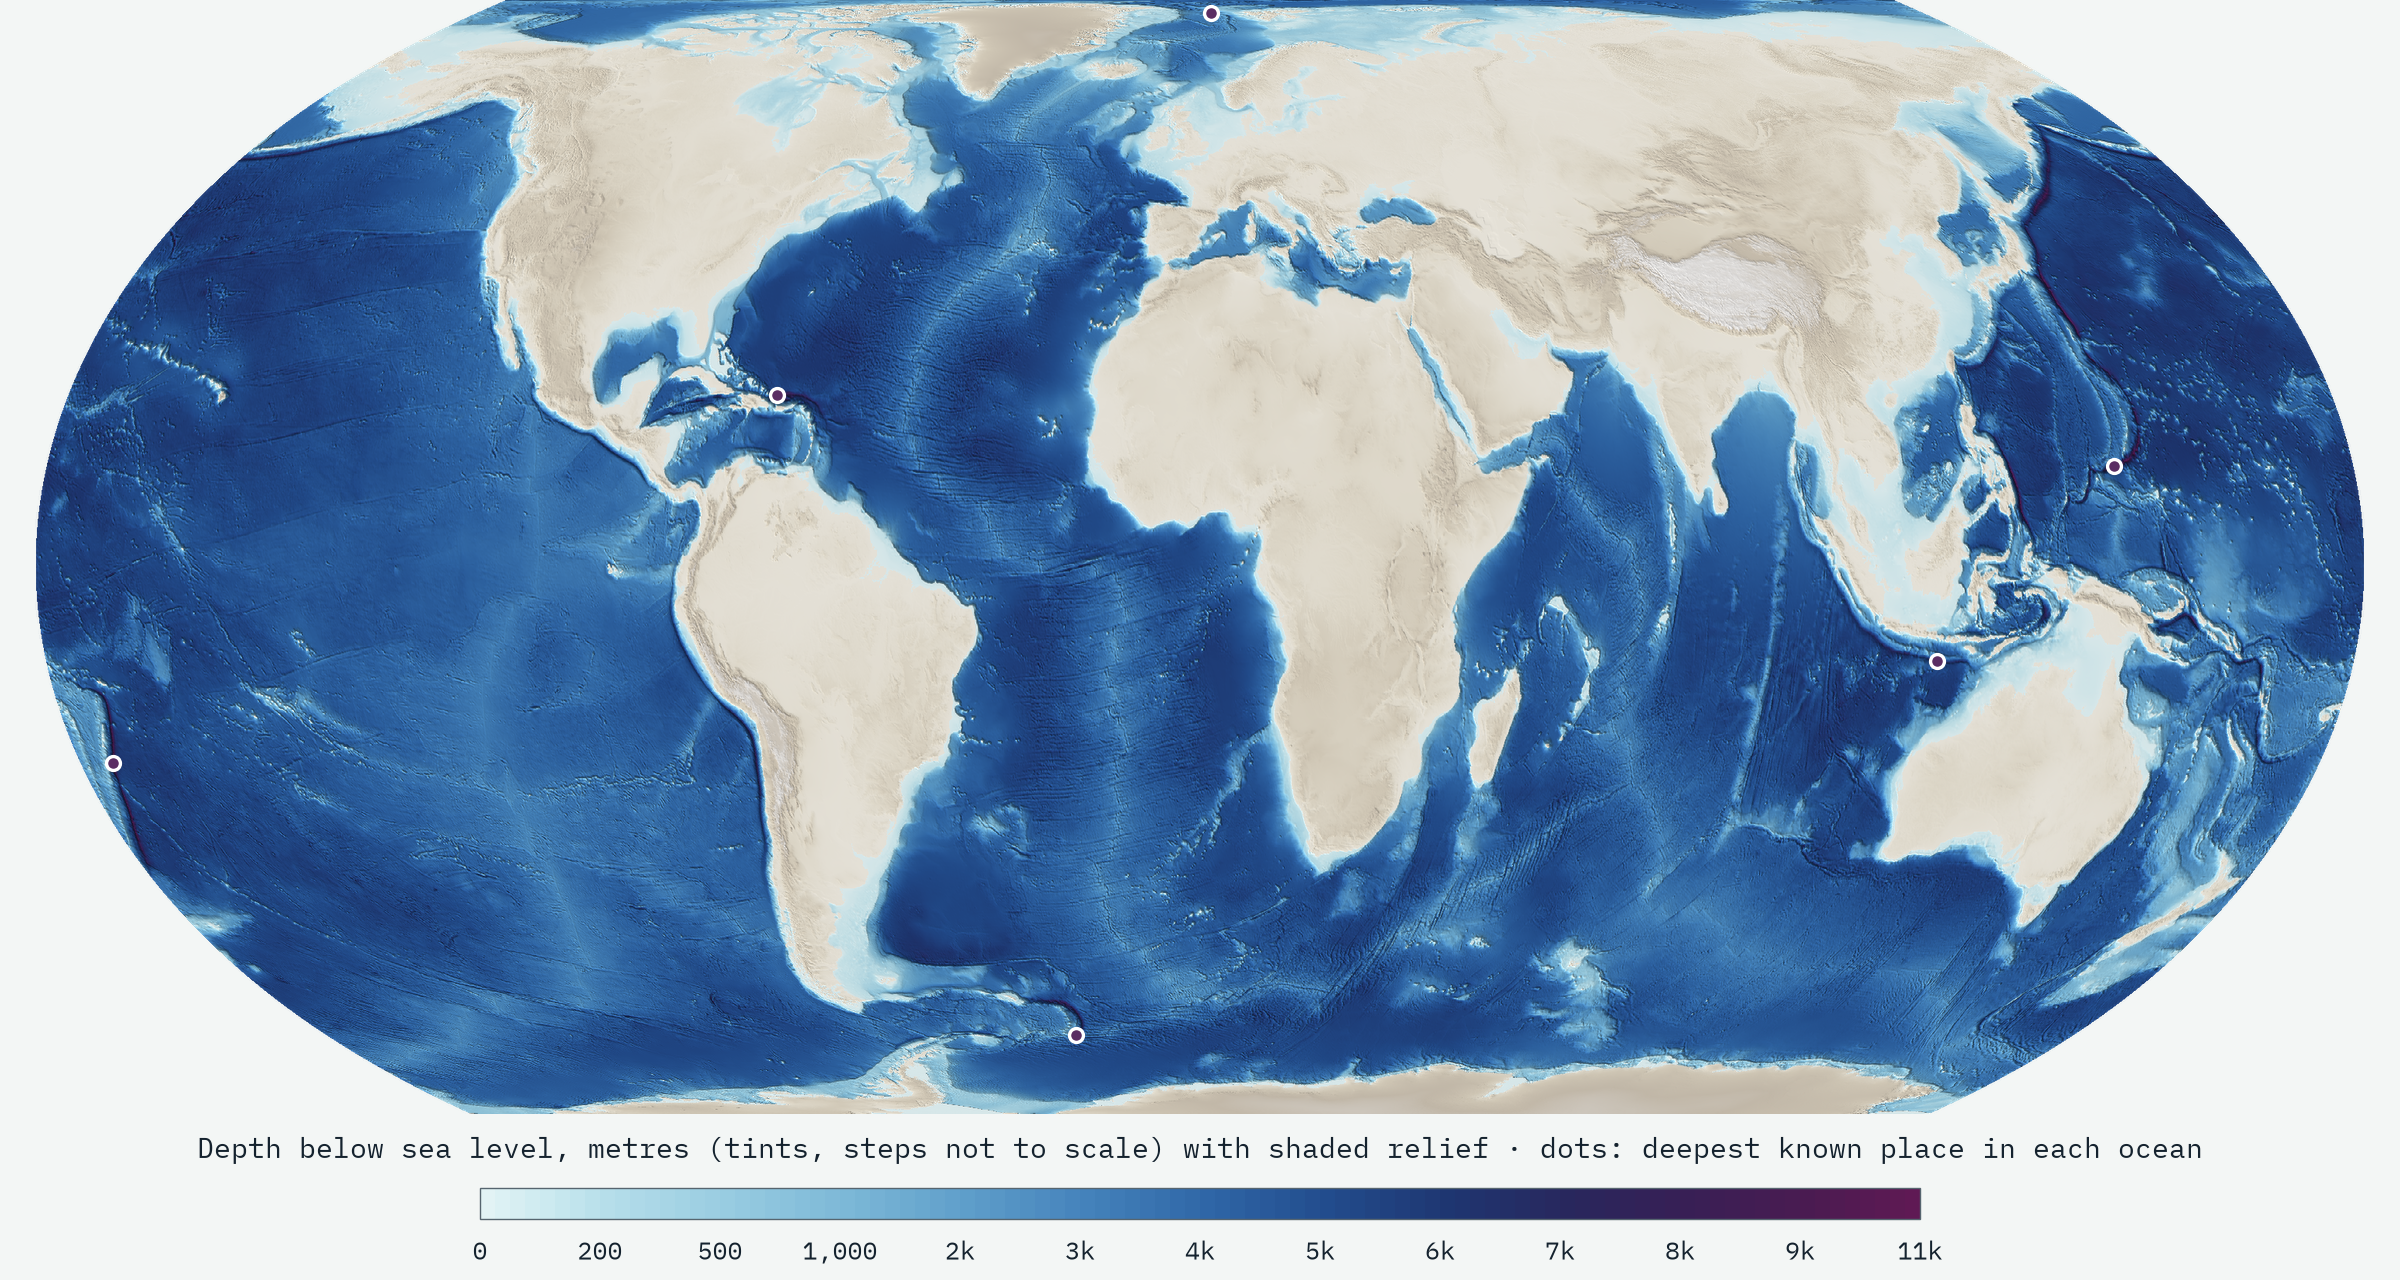
\includegraphics[width=\linewidth]{b_world_depth.png}\caption{Depth below sea level, with shaded relief, from the zoom 4 AWS Terrain Tiles resampled to 0.075 degrees and shown in the Equal Earth projection; dots mark the deepest known place in each ocean.}\label{fig:map}\end{figure}
\begin{figure}[tbp]\centering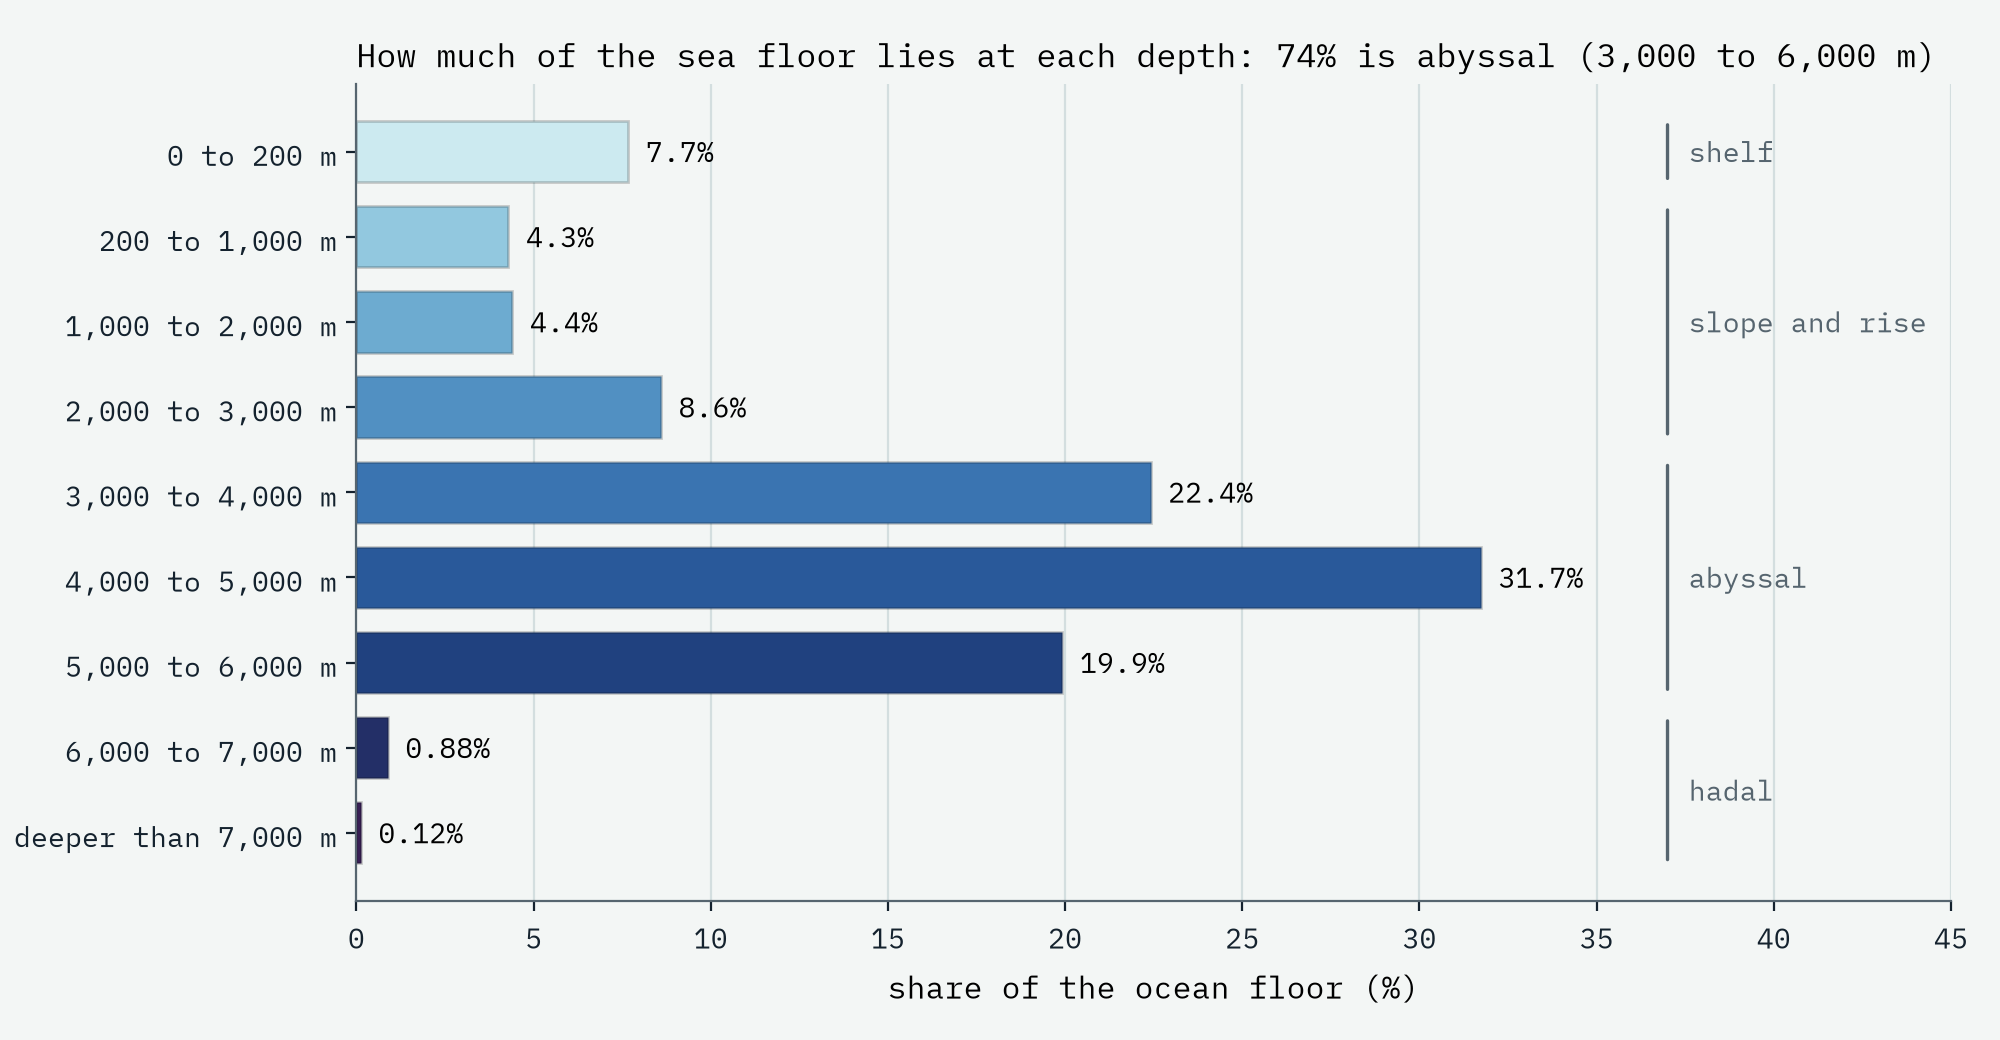
\includegraphics[width=.9\linewidth]{b_depth_bands.png}\caption{Share of the ocean floor in each depth band, with the conventional zones.}\label{fig:bands}\end{figure}

Seen across the whole Earth, the surface has two levels (Figure~\ref{fig:levels}). In 250 m steps the most common height is the lowland just above sea level, with 10.0\% of the surface between 0 and 250 m, and the second is the ocean floor between 4,500 and 4,250 m down, with 6.0\%, part of a broad mode from about 3,500 to 5,500 m. The mean sea floor lies 4.6 times deeper than the mean land stands high (801 m on the same grid). The two modes are the classic signature of two kinds of crust, thick and buoyant continental crust and thin, dense oceanic crust.

\begin{figure}[tbp]\centering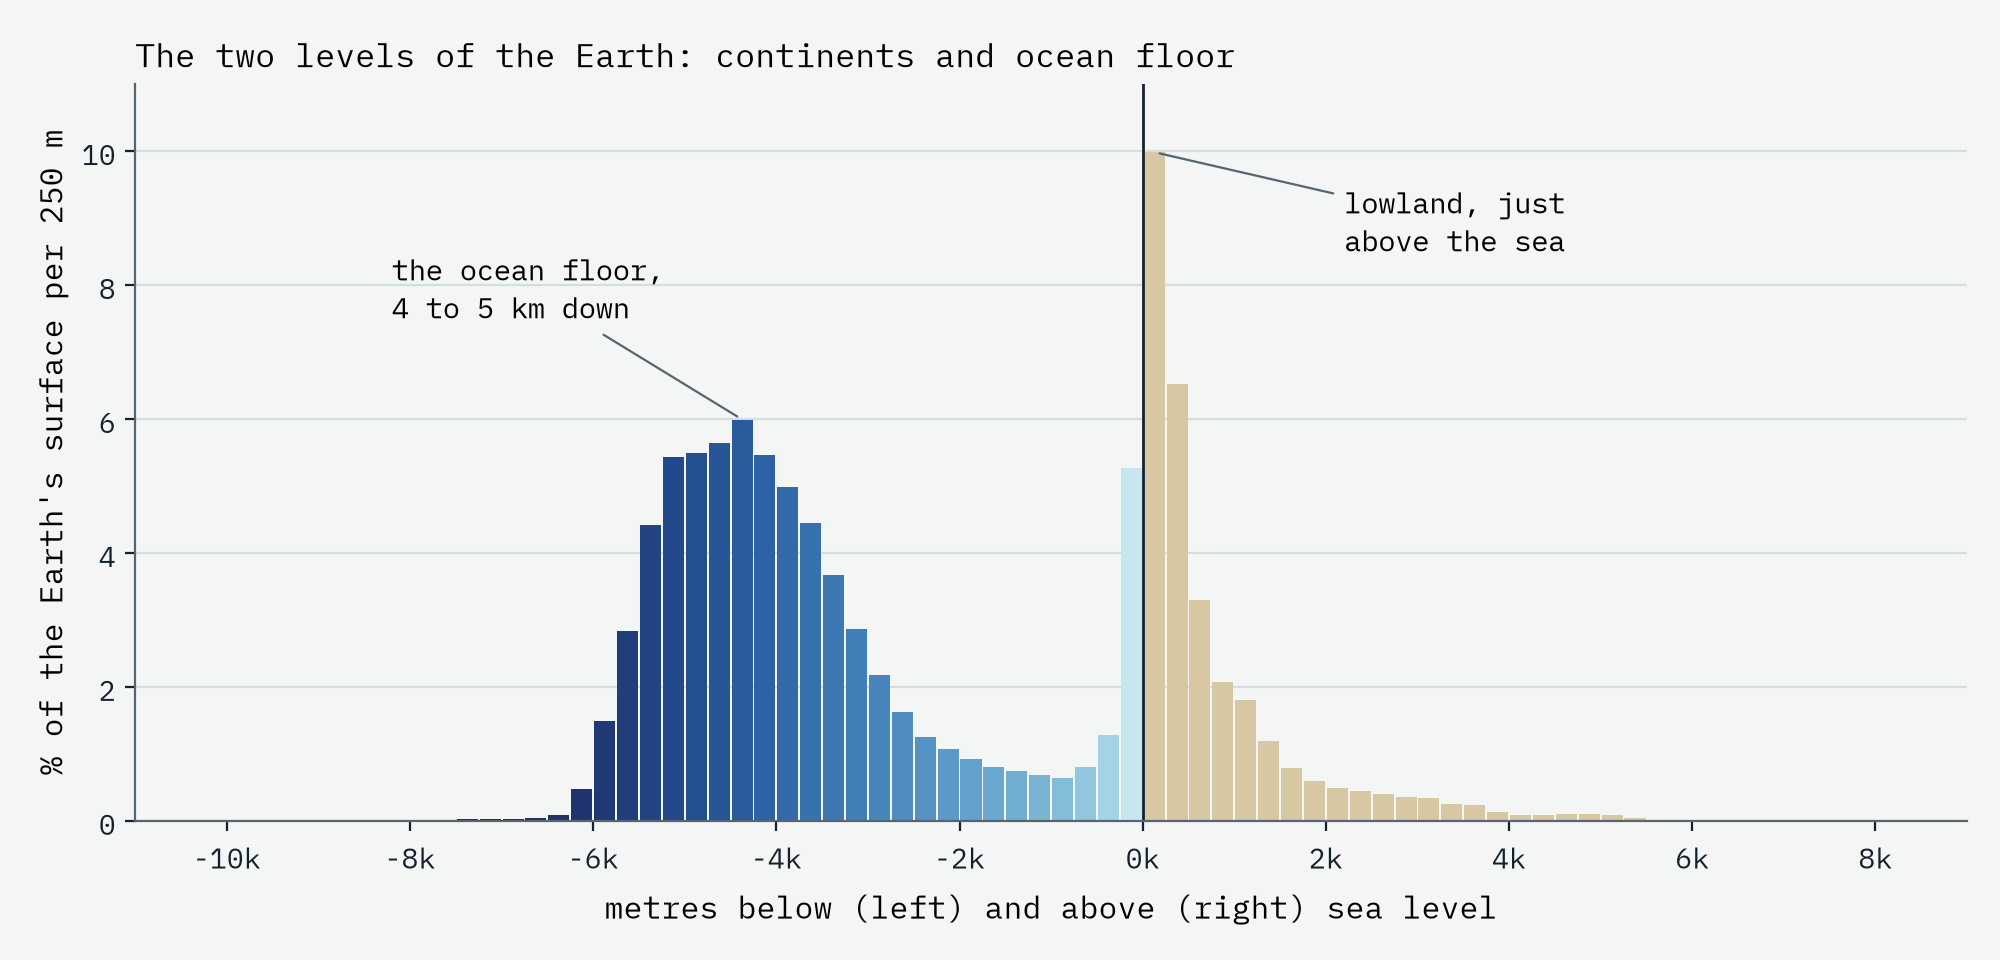
\includegraphics[width=.9\linewidth]{b_two_levels.png}\caption{Share of the Earth's surface in each 250 m step of height or depth.}\label{fig:levels}\end{figure}

\subsection{Oceans and seas}
Table~\ref{tab:oceans} and Figure~\ref{fig:oceans} give the five oceans. The Pacific holds 47\% of the sea and is the deepest on average (3,943 m), followed by the Indian (3,775 m), the Atlantic (3,606 m) and the Southern Ocean (3,213 m). The Arctic averages 1,205 m with a median of only 325 m, because 40\% of it is shelf. Among the IHO seas of more than 300,000 km² that are not oceans, the Philippine Sea is the deepest on average (4,361 m); among the shallowest are the North Sea (76 m), the Baltic (60 m), Hudson Bay (98 m) and the Persian Gulf (33 m). Every figure for each IHO sea is in \texttt{data/seas.csv}.

\begin{table}[tbp]\centering\footnotesize\setlength{\tabcolsep}{4pt}\caption{The five oceans on the zoom 4 grid: area (million km²), mean and median depth (m), shares shallower than 200 m and deeper than 6,000 m (\%), deepest grid cell (m) and the deepest measured place (m).}\label{tab:oceans}\begin{tabular}{lrrrrrrl}\toprule Ocean & Area & Mean & Median & Shelf & Hadal & Deepest cell & Deepest measured\\\midrule
Pacific & 170.2 & 3,943 & 4,256 & 5.5 & 1.65 & 10,467 & Challenger Deep, 10,935\\
Atlantic & 86.3 & 3,606 & 4,069 & 8.7 & 0.62 & 8,505 & Brownson Deep, 8,378\\
Indian & 69.9 & 3,775 & 4,091 & 4.5 & 0.43 & 7,683 & deepest point, 7,187\\
Southern & 21.9 & 3,213 & 3,805 & 8.7 & 0.01 & 6,861 & Factorian Deep, 7,432\\
Arctic & 14.7 & 1,205 & 325 & 39.8 & 0.00 & 5,657 & Molloy Hole, 5,551\\
\midrule All & 362.9 & 3,675 & 4,089 & 7.7 & 1.00 & 10,467 & Challenger Deep, 10,935\\
\bottomrule\end{tabular}\end{table}
\begin{figure}[tbp]\centering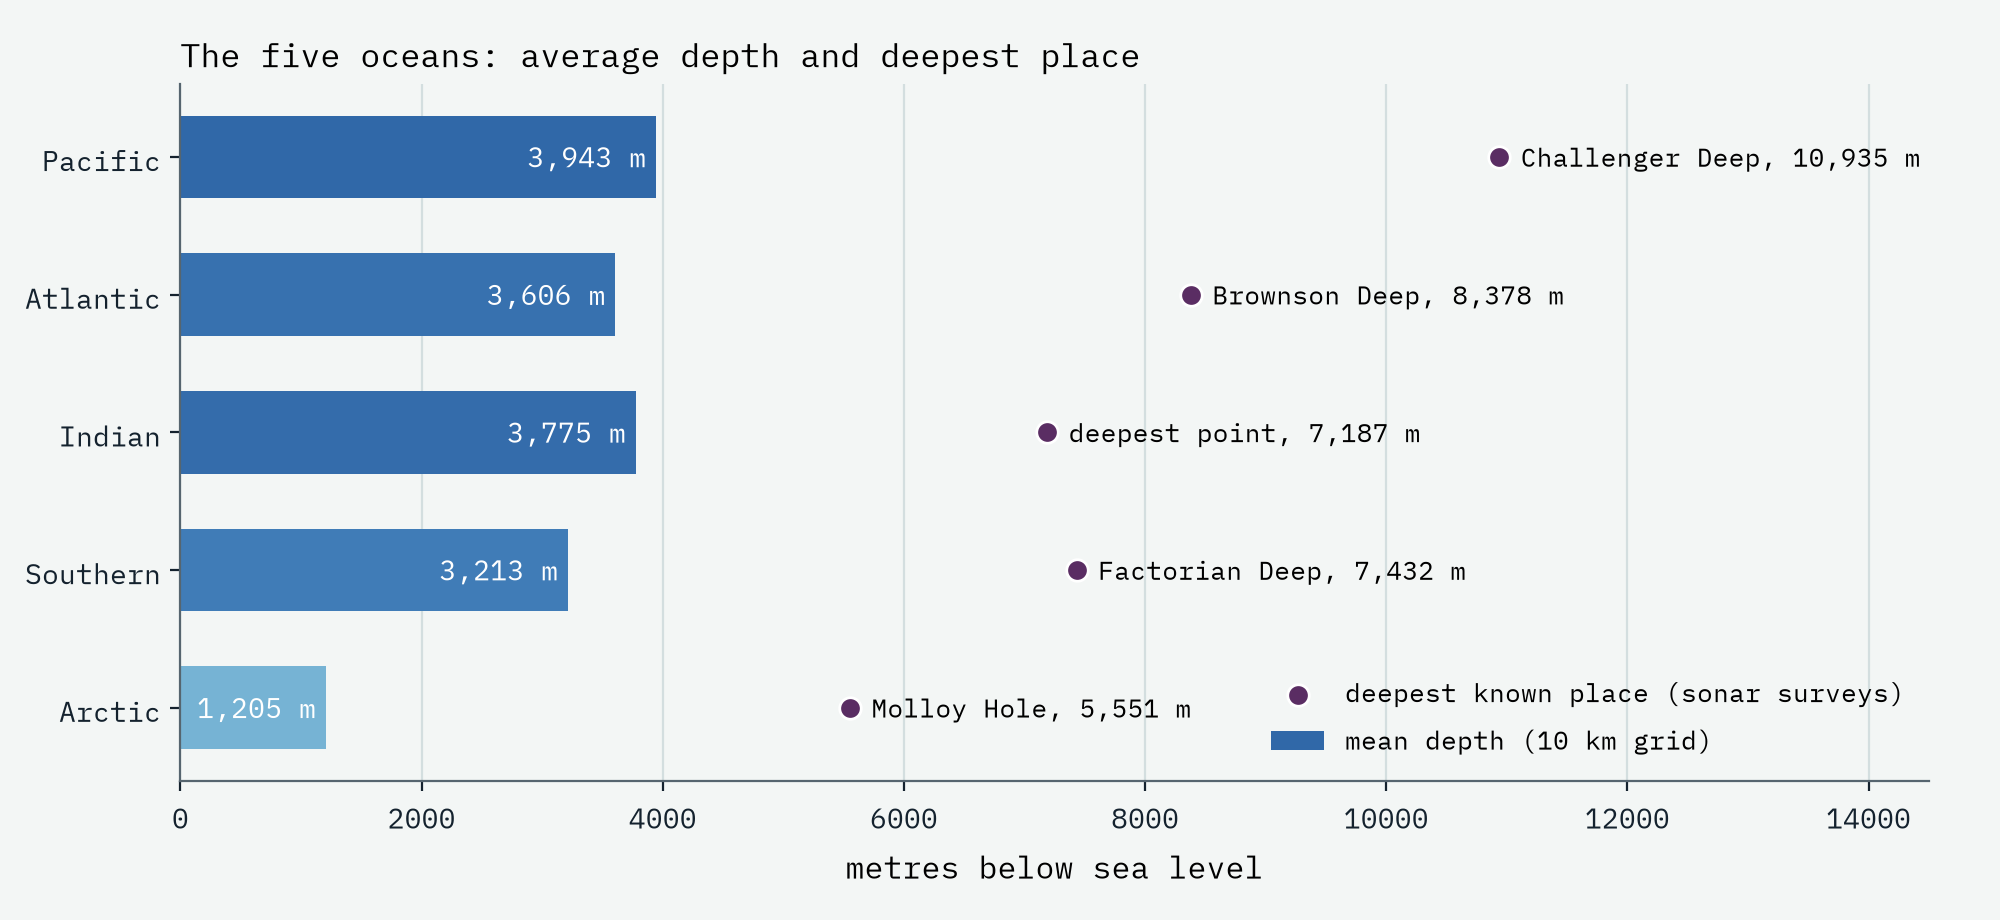
\includegraphics[width=.9\linewidth]{b_oceans.png}\caption{Mean depth of each ocean on the grid and the measured depth of its deepest known place.}\label{fig:oceans}\end{figure}

\subsection{The trenches}
Table~\ref{tab:trenches} and Figure~\ref{fig:trenches} compare the grid with published depths. The most careful estimate for the Challenger Deep, from pressure sensors on crewed submersible dives, is 10,935 $\pm$ 6 m \citep{greenaway}; the multibeam survey of \citet{bongiovanni} gave 10,924 m. Standing on the floor there, Mount Everest (8,849 m) would have 2,086 m of water above its summit (Figure~\ref{fig:mariana}).

The grid sees much less. Its deepest Mariana cell is 10,264 m, 671 m short; the cell at the published position of the Deep is 9,814 m; and the profile, which averages neighbouring cells, bottoms out at 9,931 m. The deepest cell of the whole grid, 10,467 m, lies not in the Mariana but in the Tonga Trench, 203 m deeper than the Mariana's best cell, probably because the deepest stretch of the Tonga Trench is broader, or better represented in the source grids, at the 10 km scale. The shortfall varies from trench to trench, being largest in the narrow Philippine Trench (1,041 m). In 4 places, Puerto Rico Trench, Cayman Trough, Java (Sunda) Trench and Molloy Hole, Fram Strait, the grid is deeper than anything measured. A 10 km average cannot be deeper than the deepest point within it, so these cells carry errors from old soundings or from the altimetric prediction, or, less likely, the surveys missed a deeper spot. Similar doubts surround several published depths \citep{stewart}; for the Kuril-Kamchatka Trench, for example, a later expedition failed to find depths beyond 9,500 m.

\begin{table}[tbp]\centering\footnotesize\setlength{\tabcolsep}{4pt}\caption{The deepest places: published depth and source, deepest cell of the zoom 4 grid along the trench, and the difference (m; negative where the grid is deeper).}\label{tab:trenches}\begin{tabular}{>{\raggedright\arraybackslash}p{4.2cm}>{\raggedright\arraybackslash}p{2.4cm}rlrr}\toprule Trench & Deepest point & Published & Source & Grid & Difference\\\midrule
Mariana Trench & Challenger Deep & 10,935 $\pm$ 6 & Greenaway et al. 2021 & 10,264 & 671\\
Tonga Trench & Horizon Deep & 10,816 $\pm$ 16 & Bongiovanni et al. 2022 & 10,467 & 349\\
Philippine Trench & Emden Deep & 10,540 & Wikipedia & 9,499 & 1,041\\
Kermadec Trench & Scholl Deep & 10,047 & Wikipedia & 9,604 & 443\\
Izu-Ogasawara (Bonin) Trench & deepest point & 9,810 & Wikipedia & 9,580 & 230\\
Kuril-Kamchatka Trench & deepest point & 9,604 & Wikipedia & 9,245 & 359\\
Japan Trench & deepest point & 8,412 & Wikipedia & 8,047 & 365\\
Puerto Rico Trench & Brownson Deep & 8,378 & Bongiovanni et al. 2022 & 8,505 & -127\\
South Sandwich Trench & Meteor Deep & 8,265 $\pm$ 13 & Bongiovanni et al. 2022 & 8,095 & 170\\
Peru-Chile (Atacama) Trench & Richards Deep & 8,055 & Wikipedia & 7,802 & 253\\
Cayman Trough & deepest point & 7,686 & Wikipedia & 8,071 & -385\\
South Sandwich Trench (S of 60°) & Factorian Deep & 7,432 & Bongiovanni et al. 2022 & 6,861 & 571\\
Java (Sunda) Trench & deepest point & 7,187 & Bongiovanni et al. 2022 & 7,360 & -173\\
Molloy Hole, Fram Strait & Molloy Hole & 5,551 & Bongiovanni et al. 2022 & 5,657 & -106\\
\bottomrule\end{tabular}\end{table}
\begin{figure}[tbp]\centering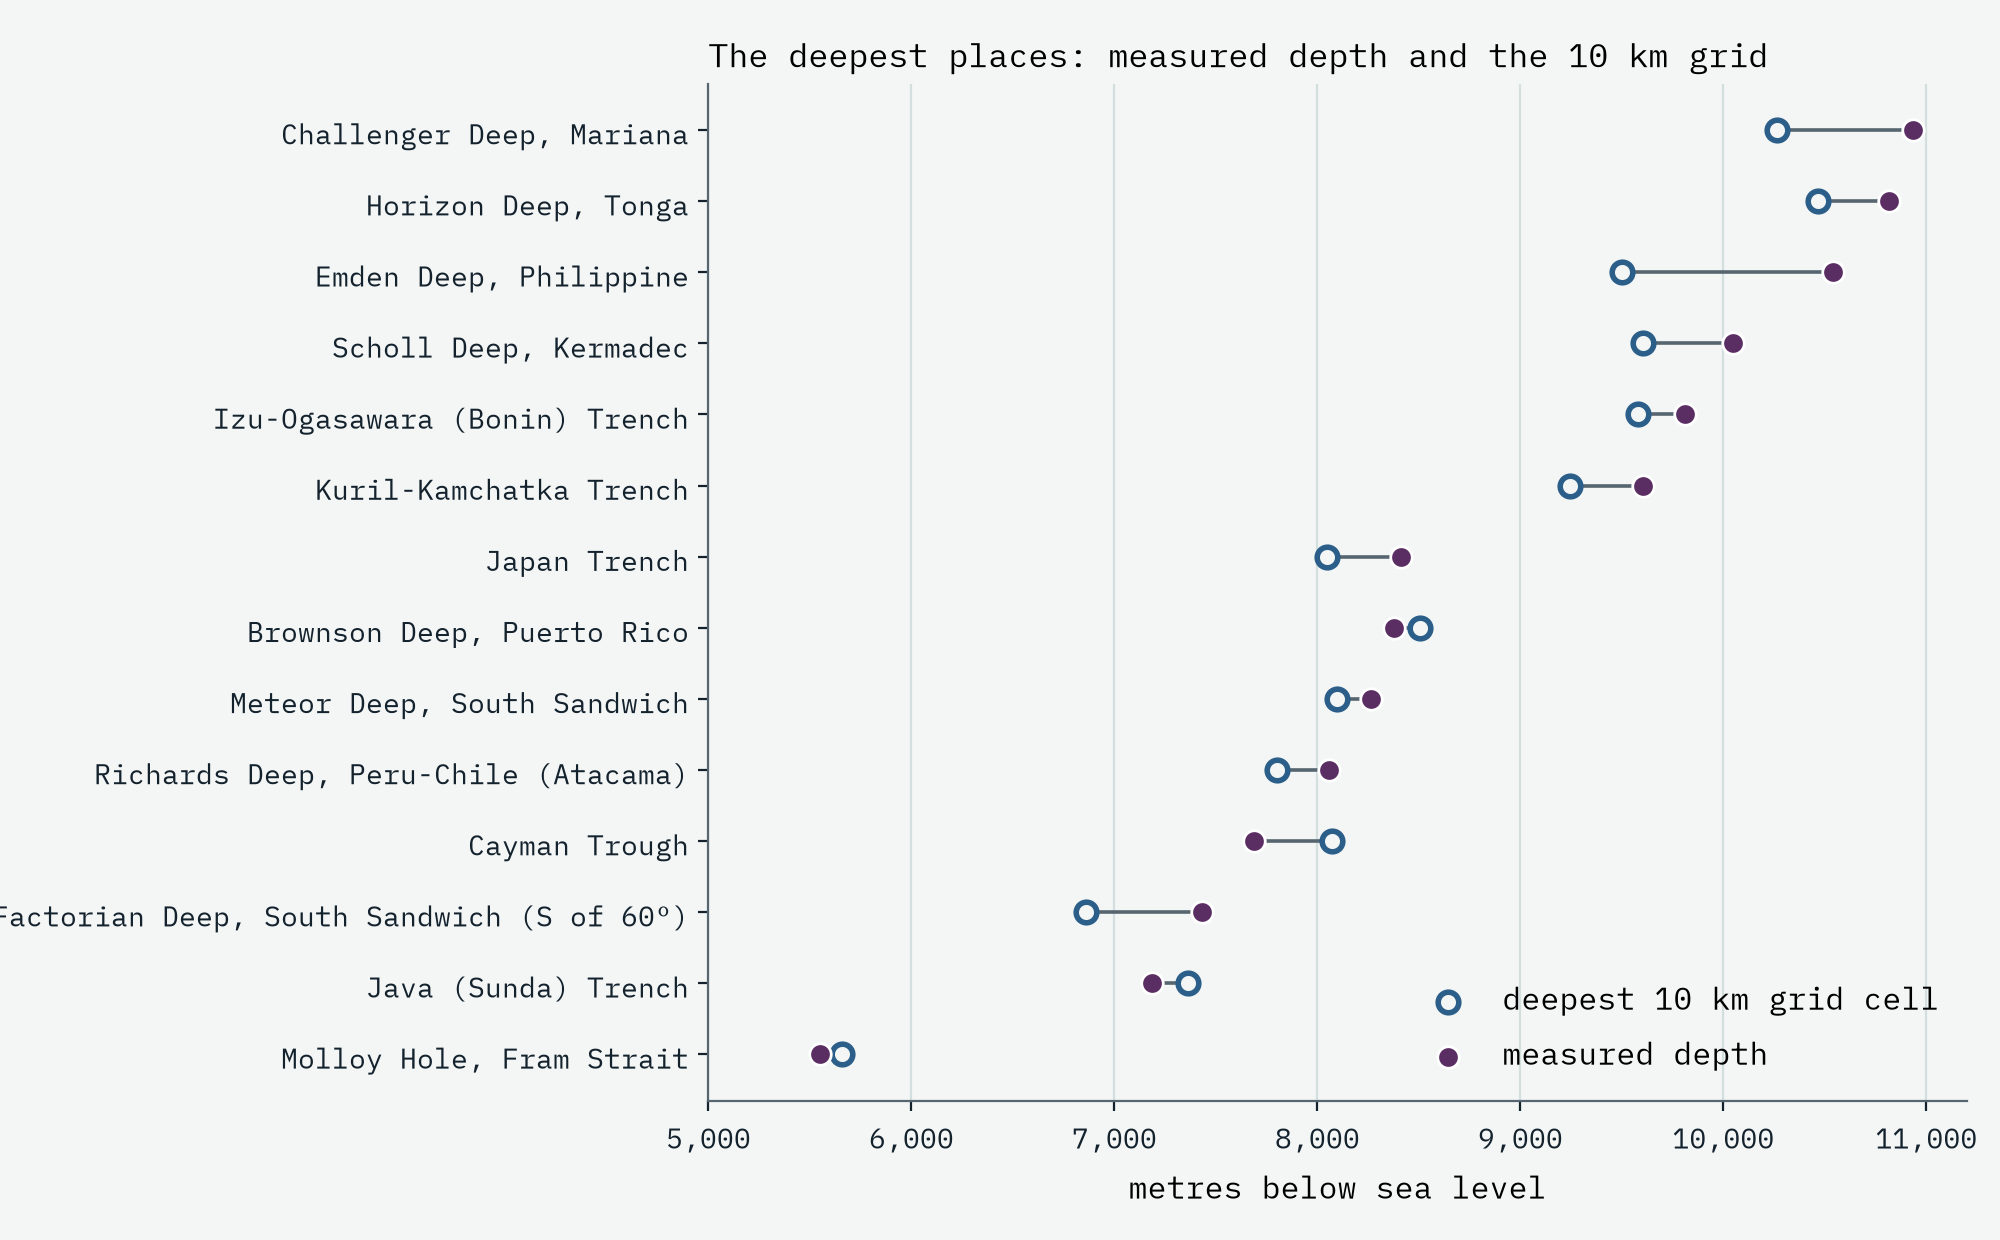
\includegraphics[width=.9\linewidth]{b_trenches.png}\caption{Measured depth of the deepest places and the deepest cell of the zoom 4 grid along each trench.}\label{fig:trenches}\end{figure}
\begin{figure}[tbp]\centering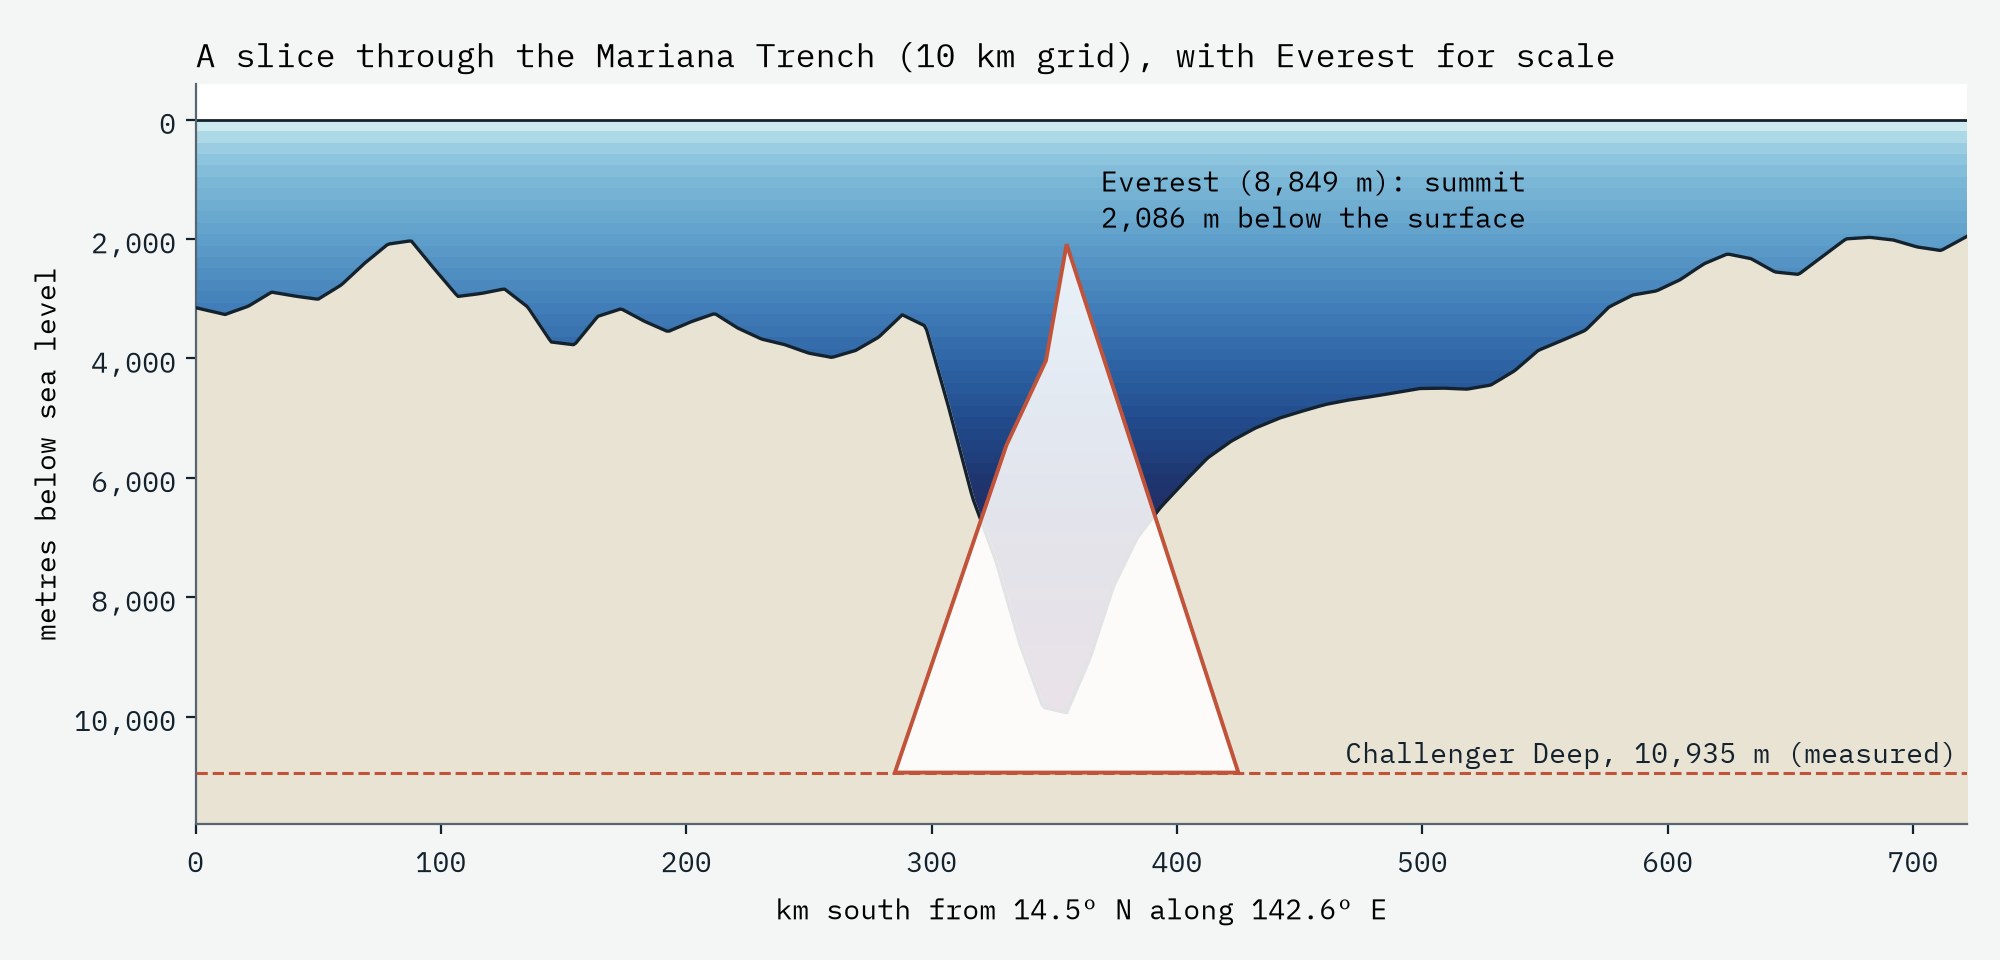
\includegraphics[width=.9\linewidth]{b_mariana.png}\caption{Profile through the Challenger Deep along 142.6° E on the zoom 4 grid, with the measured depth of the Deep (dashed) and Mount Everest drawn standing on it. Vertical scale exaggerated.}\label{fig:mariana}\end{figure}

The deepest cell in each ocean is: Pacific 10,467 m (Tonga Trench), Atlantic 8,505 m (Puerto Rico Trench), Indian 7,683 m, Southern 6,861 m (the southern end of the South Sandwich Trench) and Arctic 5,657 m (Molloy Hole). The Indian Ocean value lies not in the Java Trench but in a narrow trough at 20° S, 100.591° E in the Wharton Basin, whose depth I could not check; the deepest measured place in that ocean is in the Java Trench, 7,187 m \citep{bongiovanni}.

\subsection{National waters}
Exclusive Economic Zones, joint regimes and overlapping claims cover 38.8\% of the sea on the grid and the high seas 61.2\% (222.1 million km²). National waters are shallower on average (2,731 m against 4,273 m) because they hold the shelves, but trenches follow island arcs and continental margins, so 37\% of the sea floor deeper than 6,000 m lies within a zone. The deepest cells are in the zones of Tonga (10,467 m), the Federated States of Micronesia (10,264 m), which contains the Challenger Deep, and the United States territory of Guam (9,990 m) (Figure~\ref{fig:eez}).

\begin{figure}[tbp]\centering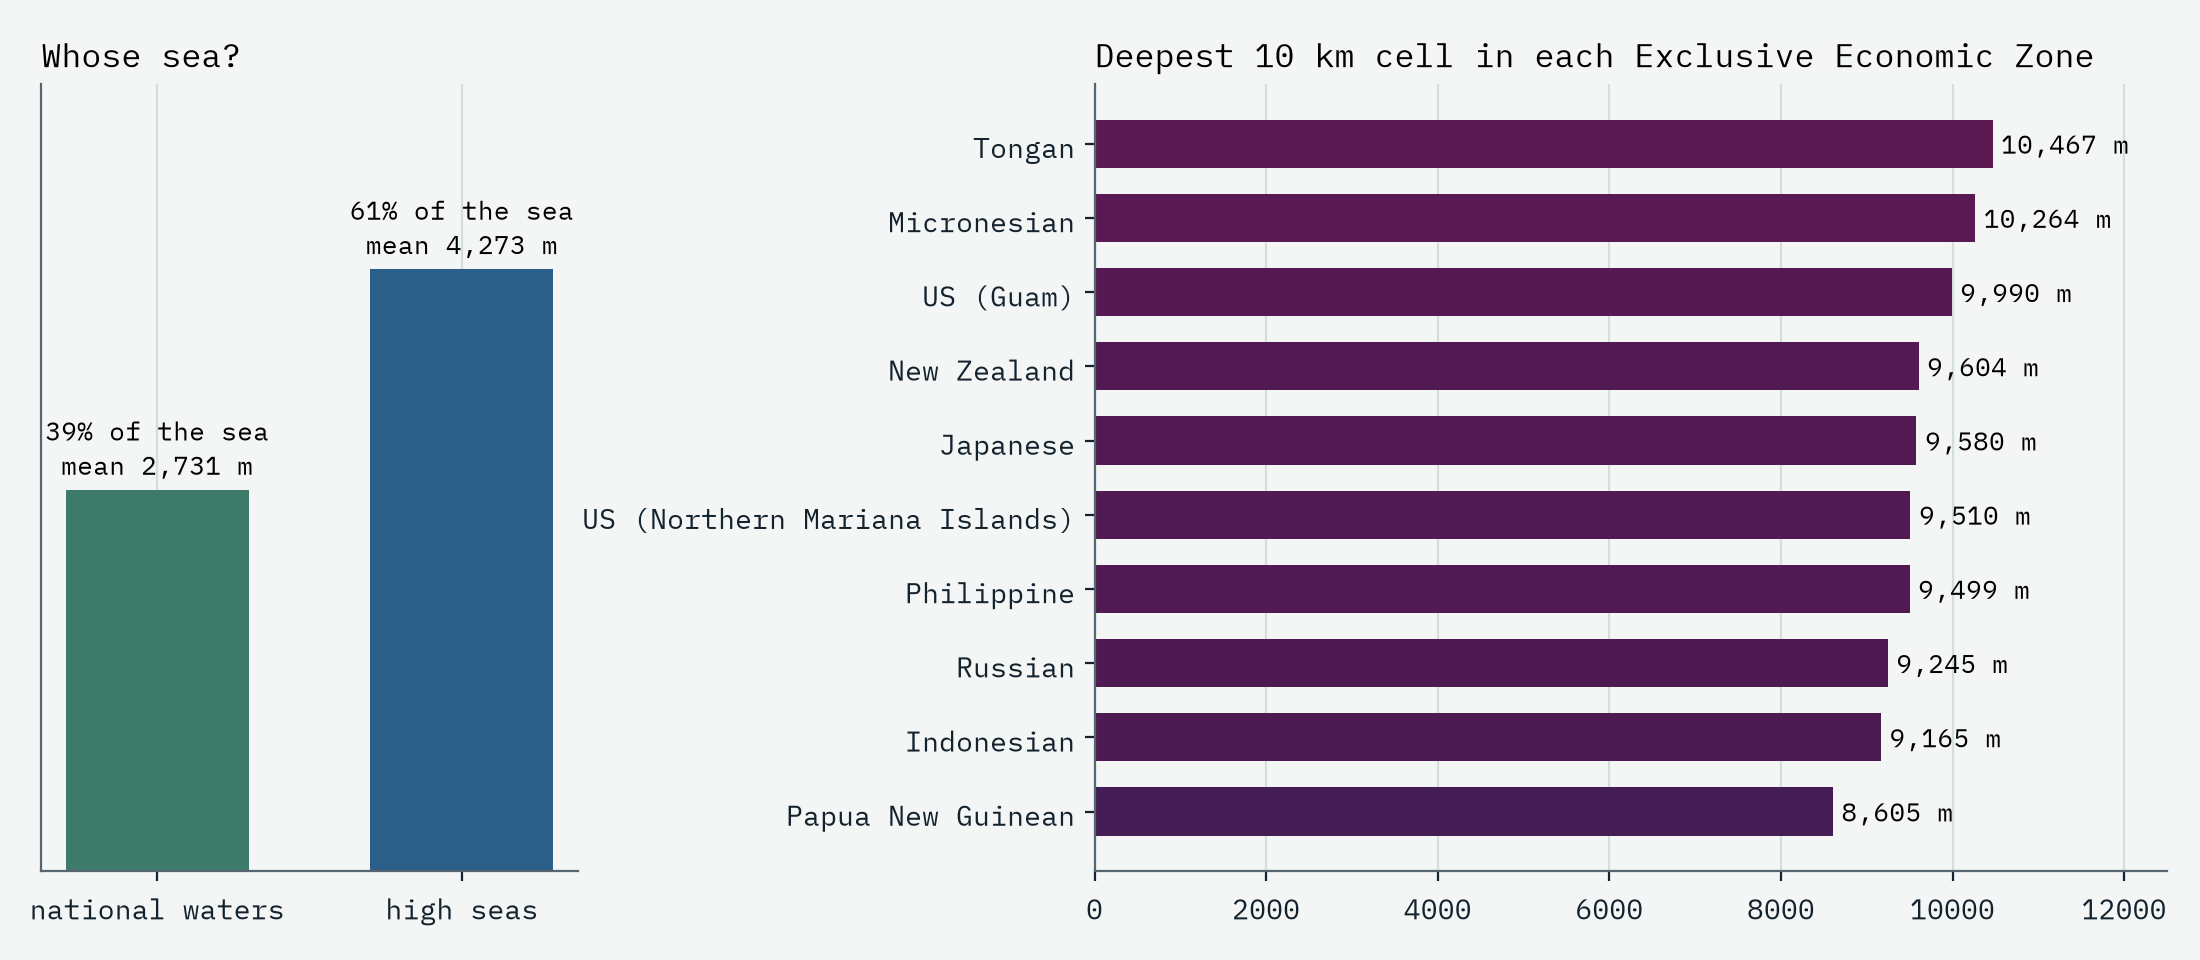
\includegraphics[width=\linewidth]{b_eez.png}\caption{Share of the sea in national waters and on the high seas, with mean depths, and the deepest grid cell in each of the ten deepest Exclusive Economic Zones.}\label{fig:eez}\end{figure}

\subsection{Seamounts and the unmapped floor}
The gazetteer's 2,549 named seamounts, guyots and knolls are about one in 9.7 of the likely seamounts identified from satellite gravity by \citet{kw2011}, and far fewer than the number of smaller ones thought to exist. The median grid depth at a named seamount's listed position is 2,902 m, but that is the depth of a 10 km cell, not of a summit. Names follow research ships, so the named features say as much about where surveys have been as about the sea floor.

That is the main limit on every number here. Seabed 2030 reported in 2026 that 28.7\% of the ocean floor is mapped to modern standards, up from 27.3\% a year before, with almost 5 million km² added in a year \citep{seabed2030, iho2026}. On this grid's ocean area that leaves about 259 million km² known only from sparse soundings and satellite prediction. At last year's gain of 1.4 percentage points a year, mapping the rest would take about 51 years; finishing by 2030 would need about 17.8 points a year.

\subsection{A check against Natural Earth}
Natural Earth's hand-drawn bathymetry gives almost the same areas as the grid at shallow thresholds and somewhat smaller ones at depth (Table~\ref{tab:ne}): the grid has 0.2\% more sea deeper than 200 m and 5.4\% more deeper than 4,000 m. The polygons generalise the deep plains inward from their edges, and at 6,000 m they cover 2.4 million km² against the grid's 3.6 million, so the hadal share is the least certain figure here.

\begin{table}[tbp]\centering\small\caption{Sea area deeper than each depth: Natural Earth's bathymetry polygons (areas on the WGS84 ellipsoid) and the zoom 4 grid (million km²).}\label{tab:ne}\begin{tabular}{rrr}\toprule Deeper than (m) & Natural Earth & Grid\\\midrule
0 & 363.2 & 362.9\\
200 & 334.4 & 335.1\\
1,000 & 317.2 & 319.5\\
2,000 & 299.9 & 303.6\\
3,000 & 266.0 & 272.4\\
4,000 & 181.2 & 191.1\\
5,000 & 67.8 & 75.9\\
6,000 & 2.4 & 3.6\\
7,000 & 0.3 & 0.5\\
8,000 & 0.1 & 0.1\\
\bottomrule\end{tabular}\end{table}

\section{Limitations}
The statistics are smoothed to about 10 km. Trenches look shallower and seamounts lower than they are, narrow straits and fjords are poorly resolved, and the shares in each band are good to about a percentage point, not to the decimal. Most of the floor in the source grids is predicted from satellite altimetry and calibrated by sparse soundings; some cells are wrong by hundreds of metres or more, as the trenches show. Sea under Antarctica's ice shelves is missing; the coastline is Natural Earth's, not the tiles'; and sea cells that average above sea level count as 0 m. The grouping of seas into oceans follows one reasonable reading of the IHO areas; others would move a few per cent of area between the Arctic and Atlantic. The Marine Regions zones are as published there and include claims that are disputed. Published depths of the deepest places come from surveys of different ages and accuracies; those taken from Wikipedia are older or less certain. The named features are only those someone has named.

\section{Conclusion}
The sea is deep: its floor averages 3,675 m and three quarters of it lies between 3,000 and 6,000 m, more than half of the planet's surface. The trenches are tiny in area but extreme in depth, and a global 10 km grid underestimates them by hundreds of metres, sometimes misplacing the deepest point altogether. All of it rests on a floor that is still mostly estimated, with 28.7\% mapped to modern standards.

\section*{Data and code availability}
The interactive map is at \url{https://maps.tristanhotham.com/ocean-depth/}. Data and code are at \url{https://github.com/Tristan-Hotham/ocean-depth} and archived with this paper at 10.5281/zenodo.23850291. Derived data are released under CC BY 4.0 and code under the MIT licence. The terrain tiles themselves are not redistributed; Marine Regions data are CC BY 4.0.

\section*{AI statement}
I wrote the text, with drafting and editing assistance from Claude (Anthropic), which also helped prepare the analysis code. I reviewed and checked all text and results.

\begin{thebibliography}{99}
\bibitem[Amante and Eakins(2009)]{etopo1} Amante, C. and Eakins, B.W. (2009) ETOPO1 1 arc-minute global relief model: procedures, data sources and analysis. NOAA Technical Memorandum NESDIS NGDC-24. National Geophysical Data Center, NOAA. doi:10.7289/V5C8276M
\bibitem[AWS(2026)]{terraintiles} Registry of Open Data on AWS (2026) Terrain Tiles. \url{https://registry.opendata.aws/terrain-tiles/}
\bibitem[Bongiovanni et al.(2022)]{bongiovanni} Bongiovanni, C., Stewart, H.A. and Jamieson, A.J. (2022) High-resolution multibeam sonar bathymetry of the deepest place in each ocean. \emph{Geoscience Data Journal}, 9(1), 108 to 123. doi:10.1002/gdj3.122
\bibitem[Charette and Smith(2010)]{charette} Charette, M.A. and Smith, W.H.F. (2010) The volume of Earth's ocean. \emph{Oceanography}, 23(2), 112 to 114.
\bibitem[Claus et al.(2014)]{marineregions} Claus, S., De Hauwere, N., Vanhoorne, B., Deckers, P., Souza Dias, F., Hernandez, F. and Mees, J. (2014) Marine Regions: towards a global standard for georeferenced marine names and boundaries. \emph{Marine Geodesy}, 37(2), 99 to 125. Data: Flanders Marine Institute (VLIZ), MarineRegions.org, CC BY 4.0, via the CatalogueOfLife col-gazetteers package.
\bibitem[GEBCO(2026)]{gebco} GEBCO Compilation Group (2026) GEBCO\_2026 Grid. General Bathymetric Chart of the Oceans. \url{https://www.gebco.net/}
\bibitem[Greenaway et al.(2021)]{greenaway} Greenaway, S.F., Sullivan, K.D., Umfress, S.H., Beittel, A.B. and Wagner, K.D. (2021) Revised depth of the Challenger Deep from submersible transects; including a general method for precise, pressure-derived depth estimates. \emph{Progress in Oceanography}, 195, 102564.
\bibitem[Hotham(2026)]{worldterrain} Hotham, T. (2026) How high is the world? Height above sea level, mountains and where people live, from open terrain data. Working paper. \url{https://maps.tristanhotham.com/world-terrain/}
\bibitem[IHO(1953)]{iho} International Hydrographic Organization (1953) Limits of Oceans and Seas, Special Publication 23, 3rd edition. Monaco. Digitised as IHO Sea Areas version 3 by VLIZ, doi:10.14284/323.
\bibitem[IHO(2026)]{iho2026} International Hydrographic Organization (2026) Global seabed mapping reaches new milestone as five million square kilometres added in a year. News release. \url{https://iho.int/}
\bibitem[Kim and Wessel(2011)]{kw2011} Kim, S.-S. and Wessel, P. (2011) New global seamount census from altimetry-derived gravity data. \emph{Geophysical Journal International}, 186(2), 615 to 631.
\bibitem[Mapzen(2017)]{joerd} Mapzen (2017) Joerd: data sources and attribution for the Terrain Tiles. \url{https://github.com/tilezen/joerd/blob/master/docs/attribution.md}
\bibitem[Natural Earth(2026)]{naturalearth} Natural Earth (2026) 1:10m cultural and physical vectors, including bathymetry and marine areas. Public domain. \url{https://www.naturalearthdata.com/}
\bibitem[Seabed 2030(2026)]{seabed2030} Nippon Foundation-GEBCO Seabed 2030 Project (2026) Release of the GEBCO\_2026 Grid: 28.7\% of the world's ocean floor mapped to modern standards. \url{https://www.gebco.net/}
\bibitem[Stewart and Jamieson(2019)]{stewart} Stewart, H.A. and Jamieson, A.J. (2019) The five deeps: the location and depth of the deepest place in each of the world's oceans. \emph{Earth-Science Reviews}, 197, 102896.
\bibitem[Tozer et al.(2019)]{srtm15} Tozer, B., Sandwell, D.T., Smith, W.H.F., Olson, C., Beale, J.R. and Wessel, P. (2019) Global bathymetry and topography at 15 arc sec: SRTM15+. \emph{Earth and Space Science}, 6, 1847 to 1864.
\bibitem[Wikipedia(2026)]{wptrench} Wikipedia contributors (2026) Oceanic trench. English Wikipedia, CC BY-SA 4.0. \url{https://en.wikipedia.org/wiki/Oceanic_trench}
\end{thebibliography}
\end{document}
